\section{Introduction partielle}
L'un des moyens permettant de se faciliter la tâche de manipulation du son, consiste à le voir comme une fonction mathématique (bien que non modélisable comme tel de manière rigoureuse). Ainsi on voit le son comme la variation d'une quantité (l'énergie de pression transmise par exemple) en fonction du temps. Cela nous permet de le traiter comme un signal parmi tant d'autres et ainsi avoir le droit d'y appliquer des résultats élaborés pour cet effet dans le cadre d'une discipline nommée \emph{traitement du signal}.\\
Le traitement du signal est en effet une discipline qui est axée sur le traitement, l'interprétation et l'analyse des signaux. Un signal peut être contrôlé, filtré, comprimé, transmis, débruité, déconvolué, identifié, classifié... C'est donc une discipline dont l'objet central d'étude est le signal (concept qui regroupe nombreux phénomènes bien particuliers comme le son, l'image,...).\\
Dans ce premier chapitre, nous abordons particulièrement les notions de base du traitement des signaux tout en orientant notre exposé dans le sens du traitement du signal qui nous concerne. Tout converge vers un traitement particulièrement utile pour notre étude, le filtrage. Nous nous focalisons sur le traitement numérique du signal vu que c'est ce qui facilite la manipulation et l'élaboration des systèmes de traitement des signaux. C'est ainsi que nous misons particulièrement sur le filtrage adaptatif bien adapté aux signaux évoluant dans le temps, ce qui est évidemment le cas de la majorité des signaux sonores.
\section{Bases théoriques du traitement du signal}
\subsection{Fondement de l'analyse des signaux\cite{KrCourse}} 
Un signal $ s(t) $ peut être vu approximativement comme une combinaison linéaire des fonctions simples et connues formant la base d'un espace vectoriel à dimension $ n $ qui est infini à la limite. Cela étant, on associera à chaque fonction $ f_i(t) $ constituant la base dudit espace vectoriel un coefficient $ \alpha_i $. Ce qui donne:
\begin{eqnarray}\label{combili}
s(t) = \sum_{i=1}^{n}\alpha_if_i(t)
\end{eqnarray}
Cette représentation des signaux est très capitale car elle facilite l'analyse du signal ainsi représenté et permet d'aborder le traitement numérique du signal. En effet, le traitement numérique d'un signal ne peut être envisagé que s'il est discrétisé or, la manière dont $ s(t) $ est écrit en \ref{combili} suggère qu'il peut se voir comme un vecteur dont les composantes sont les $ \alpha_i $, ce qui le rend en fait discret.\\
Nous venons de former un espace vectoriel des fonctions, isomorphe à $ \mathbb{R}^n $ ou à $  \mathbb{C}^n $ selon que le signal est modélisé sous la forme réelle ou complexe.

On remarque que $ s(t) $ peut être représenté par un vecteur dont les composantes changent en fonction de la famille des $ f_i(t) $ choisie. Le choix de cette famille est également primordial car c'est de lui que dépend la facilité d'analyse du signal considéré.\\
La représentation des signaux par des vecteurs est très féconde et \emph{permet par exemple d'évaluer le degré de ressemblance des signaux} grâce à la notion de distance. Pour cela, on définit une norme $ \|.\| $ sur l'espace des fonctions introduit tel que pour tout signal $ s(t) $ on ait que: 
\begin{eqnarray}\label{norme}
\|s(t)\|_{2} = \sqrt{\sum_{i=1}^{n}(\alpha_i)^2}
\end{eqnarray}\newpage
Par analogie on a que la norme de s(t) est sur une période $ \tau $:
\begin{eqnarray}\label{analogieNorme}
\|s(t)\|_{2} = \sqrt{\int_{\tau}|s(t)|^2\,dt}
\end{eqnarray}
L'expression \ref{analogieNorme} signifie que les signaux doivent être à carré intégrable. Le sens physique est que les signaux doivent avoir une énergie finie. Ce qui précède est évident pour un signal réel et constitue une condition supplémentaire à imposer à l'espace des signaux.

Soient $ s(t) = (\alpha_1,\dots,\alpha_n) $ et $ u(t) = (\beta,\dots,\beta_n) $ deux signaux, la distance entre les deux signaux sera donnée par la distance usuelle découlant de la norme définie en \ref{norme}. Soit que:
\begin{eqnarray}\label{distance}
d(s,u) &=& \|s-u\|_{2} \\
	   &=& \sqrt{\sum_{i=1}^{n}(\alpha_i-\beta_i)^2} 
\end{eqnarray}
Notez que par analogie on peut également définir, en vertu de \ref{analogieNorme}, la distance entre les signaux par:
\begin{eqnarray}
d(s(t),u(t)) = \sqrt{\int_{\tau}|s(t)-u(t)|^2\,dt}
\end{eqnarray}
La norme, telle que définie en \ref{norme}, dérive\footnote{Car on a que $ \|s\|=\sqrt{\langle s,s \rangle} $} évidemment d'un produit scalaire\cite{TopoHilb}; ce produit est donné par:
\begin{eqnarray}
\langle s,u \rangle = \sum_{i=1}^{n}(\alpha_i.\beta_i^{\star})
\end{eqnarray}
Avec $ \beta_i^{\star} $ le complexe conjugué de $ \beta_i $ pour être plus général.\\
Comme habituellement nous pouvons aussi définir ce produit pour les signaux non discrétisés sur une période de temps $ \tau $ par:
\begin{eqnarray}
\langle s(t),u(t )\rangle = \int_{\tau}(s(t).u^{\star}(t))\,dt
\end{eqnarray}
Le produit scalaire de deux vecteurs est proportionnel à la projection de l'un sur l'autre. Il est maximum, en valeur absolue, lorsque les deux vecteurs ont la même orientation et nul lorsqu'ils sont orthogonaux. Il peut donc être considéré comme une mesure de la similitude d'orientation des vecteurs. En d'autres termes, le rapprochement des signaux dans leur évolution (similitude des formes).


L'espace vectoriel des fonctions ainsi défini et muni de ce produit scalaire qui y induit une norme est \emph{complet}\cite{TopoHilb} et constitue \emph{un espace de Hilbert}. La connaissance de cette structure est cruciale car elle permet de traiter tous les éléments de cet espace des signaux en utilisant juste les résultats connus sur les espaces de Hilbert.

Ce qui vient d'être démontré justifie que les signaux soient développables  en série des fonctions orthogonales et non liées. D'où la possibilité de les développer en \emph{série de Fourier} ou bien en considérant les autres familles des fonctions orthogonales selon les besoins et la commodité. Le développement en série de Fourier est en fait d'une importance capitale en théorie du signal.
\subsection{Signaux déterministes}
Les signaux déterministes sont ceux représentables par une fonction analytique. Suite à ce qui vient d'être montré à la sous-section précédente, nous allons reconsidérer la transformée de Fourier dans cette partie et en aborder les aspects utiles à notre travail.
La transformation de Fourier est vue comme une généralisation du développement en série des fonctions orthogonales de Fourier tel que présenté dans la partie qui précède.
Le développement en série Fourier est donnée par \cite{Piskounov}:
\begin{eqnarray}\label{SrFourier}
s(t) = \sum_{n = -\infty}^{+\infty}[S_{n}.e^{j2{\pi}nft}]
\end{eqnarray}
Cette équation constitue donc, à quelques changements de variable près, un cas particulier de \ref{combili}.
Avec les coefficients $ S_{n} $ donnés par:
\begin{eqnarray}\label{CoefFourier}
S_{n}=\frac{1}{T}.\int_{\frac{-T}{2}}^{\frac{T}{2}}s(t).e^{-j2{\pi}nft}\,dt
\end{eqnarray}\newpage
\subsubsection{Définition \cite{KrCourse}}
Soit $ s(t) $ un signal déterministe, sa transformée de Fourier $ \mathbb{S} $ est définie par:
\begin{eqnarray}\label{TrFourier}
\mathbb{S}(f) = \int_{-\infty}^{+\infty}s(t).e^{-j2\pi ft}\,dt
\end{eqnarray}
Avec $ t $ la variable \emph{temps} et $ f $ la \emph{fréquence}. Ce qui induit une dualité temps-fréquence, le passage de l'un des domaines à l'autre étant réalisable par symétrie vu que la transformée inverse de Fourier est donnée par:
\begin{eqnarray}\label{TrInvFourier}
s(t) = \int_{-\infty}^{+\infty}\mathbb{S}(f).e^{j2\pi ft}\,df
\end{eqnarray}
\subsubsection{Intérêt de la transformation ainsi définie}\label{InteretFourier}
On démontre que l'une des conditions pour qu'une fonction $ f(t) $ soit développable en série de fonctions orthogonales trigonométriques (série de Fourier) est qu'elle soit périodique, et pourtant dans la majorité des situations ce n'est pas le cas.\\
Ici nous comptons montrer qu'à une fonction quelconque correspondra une \emph{transformée de Fourier}\footnote{Évidemment, si ladite fonction est à carré sommable, c'est-à-dire si son carré a une intégrale finie.}. Pour cela, considérons un signal quelconque $ s(t) $ et ciblons-y une région simple dont on connait l'expression analytique. Supposons ensuite un signal $ s_{1}(t) $ qui serait une réplique à l'infini de la partie ciblée. $ s_{1}(t) $ est par cela périodique de période $ t_{f}-t_{i} $ avec $ t_{f} $ l'instant final de la partie ciblée et $ t_{i} $ son instant initial.\\
Suite à cette définition de $ s_{1}(t) $, il est évident qu'en prenant $ T $ (c'est-à-dire $ t_{f}-t_{i} $) \emph{infinie}, cela revient à prendre $ s(t) $. D'où:
\begin{eqnarray}
s(t) = \lim_{T \to +\infty} s_{1}(t)
\end{eqnarray}
Nous savons pourtant que le développement de $ s_{1}(t) $ en série de Fourier existe car elle est périodique. Il sera donné mutatus mutandi par les rélations \ref{SrFourier} en prenant en compte \ref{CoefFourier}. Par conséquent,la représentation fréquentielle de $ s_{1}(t) $ est un spectre des raies et la distance entre raies adjacentes vaut $ f_{1} = \dfrac{1}{T} $ étant donné que le développement en série de Fourier suggère que toutes les fréquences, dans le développement de $ s_{1}(t) $, sont multiples de $ f_{1} $. La densité spectrale de raies sera alors donnée par, suite à la relation \ref{CoefFourier}:
\begin{eqnarray}\label{DensiteSpectrale}
\frac{{S_{1}}_{n}}{f_{1}} = T.{S_{1}}_{n} = \int_{\frac{-T}{2}}^{\frac{T}{2}}s_{1}(t).e^{-j2{\pi}nf_{1}t}\,dt
\end{eqnarray}
Ainsi donc, les raies deviennent de plus en plus rapprochées à mesure que $ T $ croît et à l'infini, la somme donnée en \ref{SrFourier} se transforme en une intégrale et $ f_{1} $ devient infinitésimale, ce qui fait que:
\begin{align*}
s(t) &= \lim_{T \to +\infty} s_{1}(t)\\
&= \lim_{T \to +\infty} \{\sum_{n = -\infty}^{+\infty}\frac{1}{T}.[\int_{-\frac{T}{2}}^{\frac{T}{2}}(s_{1}(t).e^{-j2{\pi}nf_{1}t}\,dt)].e^{j2{\pi}nf_{1}t}\}\\
&= \int_{-\infty}^{+\infty}\,df.[\int_{-\infty}^{+\infty}s(t).e^{-j2{\pi}ft}\,dt)].e^{j2{\pi}ft}\\
&= \int_{-\infty}^{+\infty}\mathbb{S}(f).e^{j2{\pi}ft}\,df
\end{align*}
Ceci exprime très clairement qu'un signal s(t) quelconque peut être vu comme la transformée inverse de sa transformée de Fourier. Cela prouve qu'il existe, sous certaines hypothèses(voir la note de bas de page précédente), une fonction fréquentielle $ \mathbb{S}(f) $ exprimant le signal $ s(t) $ dans le domaine des fréquences. C'est évidemment clair étant données les relations \ref{TrFourier} et \ref{TrInvFourier}.\\
Nous en déduisons que la transformée de Fourier représente, à la limite, la densité spectrale de raies telle que définie en \ref{DensiteSpectrale}.
D'où l'intérêt de cette transformée, généralisant le développement en série de Fourier, grâce à l'extension aux fonctions non périodiques.
\subsection{Signaux aléatoires}
\paragraph{}
Les signaux déterministes, sont, comme nous venons de le voir, des fonctions telles que, à chaque instant, on dispose d'une règle permettant d'en évaluer la valeur. Cette règle peut être spécifiée sous forme d'une expression mathématique,ou d'une équation récurrente ou tout autre procédé de construction.
Les fonctions déterministes forment la base de l'analyse mathématique, mais la plupart de phénomènes que nous aurons à modéliser ne sont pas de cette nature.\newpage
\begin{center}
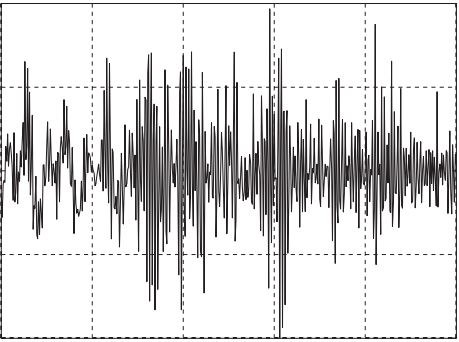
\includegraphics[scale=1]{SignalParole.jpg}
\captionof{figure}{Visualisation d'un signal de parole sur une durée de 1/16 de seconde \cite{Tsa}}
\label{FigParole}
\end{center}
Considérons le signal de parole représenté à la figure \ref{FigParole}. Il est clair, à la vue de ce graphe, que l'on ne peut réduire ces observations à une fonction déterministe du temps. Nous pourrions peut-être trouver une fonction déterministe qui approxime correctement les valeurs observées sur un intervalle de temps $ [0,T] $, mais cette fonction ne serait pas une approximation valable de l'observation à l'extérieur de cet intervalle, et cette propriété perdurerait indépendamment de la durée $ [0,T] $ de l'observation. Le graphe \ref{FigParole} contient un très grand nombre d'irrégularités et ces irrégularités ne semblent pas respecter une évolution prédictible. Les observations ont un caractère aléatoire, dans le sens où nous ne savons pas déterminer, pour un instant donné, quelle sera la valeur précise de la mesure. Par contre, il est envisageable d'indiquer un intervalle de valeurs possibles et éventuellement de préciser comment ces valeurs sont distribuées à partir d'une certaine loi de probabilité.\\
La bonne façon de décrire le comportement du phénomène est donc de spécifier, à chaque instant, une distribution de probabilité, permettant de décrire la vraisemblance de chaque observation. Dans le langage des probabilités, la valeur observée sur le capteur à chaque instant est une variable aléatoire et son évolution au cours du temps, un processus aléatoire. Cet exemple est le prototype d'une large classe de phénomènes qui conduit à adopter, pour les modéliser, la prise en compte de l'indéterminisme \cite{Tsa}.
\paragraph{}
Les signaux aléatoires sont donc en bref des signaux dont la valeur instantanée est imprévisible, ce qui implique qu'ils n'ont pas de représentation analytique. Ces signaux seront étudiés grâce à certains paramètres statistiques qui leur sont associés. C'est en fait ces types de signaux qui sont rencontrés dans notre contexte et nous en reparlerons de manière plus approfondie, mais implicite, dans les parties qui vont suivre.
\subsection{Cas des signaux discrets}
Nous aborderons ici les signaux discrets de manière secondaire. C'est-à-dire, en les prenant comme le résultat de l'\emph{échantillonnage} d'un signal continu, vu que c'est cet aspect qui nous intéressera dans le présent travail.
\subsubsection{Echantillonnage}
Echantillonner\footnote{C'est l'une de manières les plus simples de discrétiser un signal} un signal consiste à prélever, à intervalle de temps régulier le plus souvent, les valeurs prises par le signal. Cela permet ainsi de voir le signal comme une suite de nombres et en permet le traitement par un ordinateur ou tout autre système de traitement des données. C'est en fait le processus de \emph{conversion analogique-numérique}.\\
De manière formelle donc, si on prélève les valeurs du signal avec une période $ T_{e} $, on aura une suite des nombres valant $ \{ s(nT_{e}) \}_{n \in \mathbb{Z}} $ \footnote{De manière tout à fait générale, sans prendre en compte dans un premier temps la causalité (c'est-à-dire le fait selon lequel le temps doit uniquement être pris positif)} qui constitue les échantillons du signal. Par ce fait même, on est amené à songer au problème de reconstitution du signal à partir de ses échantillons. Avant de considérer ce problème, définissons l'impulsion de Dirac qui nous sera très utile pour la suite du travail même si elle n'est pas physiquement réalisable de manière parfaite car elle est idéale.
\paragraph{Impulsion de Dirac\cite{TraitSignMath} :}
Un Dirac $ \delta(t) $ est par définition \emph{une distribution} dont le support (domaine non nul) est réduit au point $ t = 0 $ et d'intégrale valant 1. Formellement, il est défini par:
\begin{eqnarray}
\int_{-\infty}^{+\infty}\delta(t)\,dt = 1
\end{eqnarray}
Ce qui veut dire que cela correspond à un signal de durée nulle et de surface $ 1 $. C'est en fait une limite définie pratiquement par \cite{Unified}:
\begin{eqnarray}
\delta(t) = \lim_{T \to 0}
\begin{cases}
\dfrac{1}{T} & \text{  pour  $ \lvert \dfrac{t}{T} \rvert <\dfrac{1}{2} $}\\
0 & \text{  pour  $ \lvert \dfrac{t}{T} \rvert >\dfrac{1}{2} $} 
\end{cases}
\end{eqnarray}
De cela on peut montrer que:
\begin{eqnarray}
\int_{-\infty}^{+\infty}s(t).\delta(t)\,dt = s(0)
\end{eqnarray}
Comme $ \delta(t-\tau) $ représente une impulsion de Dirac localisée plutôt en $ \tau $, on aura que:
\begin{eqnarray}\label{FonctionVsDirac}
\int_{-\infty}^{+\infty}s(t).\delta(t-\tau)\,dt = s(\tau)
\end{eqnarray}
On remarque que cette manipulation permet de prélever des valeurs de $ s(t) $ en des instants $ \tau $ bien précis. Plus généralement, introduisons un opérateur complet d'échantillonnage nommé \emph{peigne de Dirac} (plusieurs Dirac étendus sur toute la droite des réels et espacés chaque fois de $ \tau $ secondes). Il sera donné par:
\begin{eqnarray}\label{peigneDirac}
c(t) = \sum_{n=-\infty}^{+\infty}\delta(t-n\tau)
\end{eqnarray}
$ c(t) $ permet de réaliser complètement l'échantillonnage d'un signal $ s(t) $ car avec lui on prélève à intervalle de temps régulier $ \tau $ (période d'échantillonnage), la valeur correspondante du signal. En effet, le signal échantillonné est alors donné par \emph{la distribution}:\\
$ s_{e}(t) = \sum_{n=-\infty}^{+\infty}s(nT_{e})\delta(t-nT_{e})
= \sum_{n=-\infty}^{+\infty}s(t)\delta(t-nT_{e})
= s(t)\sum_{n=-\infty}^{+\infty}\delta(t-nT_{e}) $\\
En bref, au vu du développement qui vient d'être fait, on a:
\begin{eqnarray}\label{SignEchantillonDirac}
s_{e}(t) = s(nT_{e}) = s(nT_{e}).c(t) = s(t).c(t)
\end{eqnarray}
Echantillonner un signal revient donc juste à le multiplier par le peigne de Dirac.
\paragraph{Condition d'échantillonnage correct:}
La reconstitution du signal à partir de ses échantillons n'est réalisable que sous certains critères dont le \emph{théorème d'échantillonnage} dit \emph{théorème de Nyquist-Shannon}. Ce théorème donne une condition sur le support du spectre (donné par la transformée de Fourier) du signal $ s(t) $ pour reconstituer $ s(t) $ à partir de ses échantillons $ s(nT_{e}) $. Ce théorème est ainsi énoncé \cite{beal2012theorie}:
\begin{theorem}[Nyquist-Shannon]\label{TheoShannon}
Soit $ s(t) $ un signal dont la transformée de Fourier $ \mathbb{S}(\omega) $\footnote{$ \omega $ représentant la pulsation du signal, avec $ \omega=2.\pi.f $} est à support dans $ [-\frac{\pi}{T_{e}},\frac{\pi}{T_{e}}] $. Alors $ s(t) $ peut être reconstruit en interpolant sur ses échantillons
\begin{eqnarray}
s(t) = \sum_{n=-\infty}^{+\infty}s(nT_{e}).h_{T_{e}}(t-nT_{e})
\end{eqnarray}
Avec
\begin{eqnarray}
h_{T} = sinc(\frac{{\pi}t}{T}) = \frac{\sin\frac{\pi t}{T}}{\frac{\pi t}{T}}
\end{eqnarray}
\end{theorem}
Le théorème nous donne une condition sur  $ \omega $ pour que la reconstitution du signal à partir de ses échantillons soit possible. Cette condition est en effet $ | \omega | \leq \frac{\pi}{T_{e}} $ ce qui veut dire que la fréquence devra vérifier $ f_{max} \leq \dfrac{f_{e}}{2} \Rightarrow f_{e} \geq 2.f_{max} $. En bref, le théorème \ref{TheoShannon} nous dit que \emph{la reconstitution du signal à partir de ses échantillons n'est possible que si la fréquence d'échantillonnage $ f_{e} $ est supérieure ou égale au double de la fréquence maximale du spectre associé au signal}.
\subsubsection{Transformée de Fourier \cite{TraitSignMath}}
Pour un signal discret $ s(nT_{e}) $, la transformée de Fourier est définie par :
\begin{eqnarray}
\mathbb{S}_{d}(f) = \sum_{n = -\infty}^{+\infty}s(nT_{e}).e^{-i.2 \pi f.n}
\end{eqnarray}
C'est au fait la transformée de Fourier de sa représentation sous forme de distribution telle que donnée par \ref{SignEchantillonDirac}.\\
On sait pourtant qu'à un point de vu réel on n'a qu'un nombre fini $ N $ d'échantillons. Pour prendre cela en compte, on définit la transformée de Fourier pour le cas des \emph{signaux finis}. Elle est évidemment donnée par:
\begin{eqnarray}\label{TrFourFinie}
\mathbb{S}_{d}(f) = \sum_{n = 0}^{N-1}s(nT_{e}).e^{-i \frac{2 \pi n}{N} f}
\end{eqnarray}
Cela veut dire que la transformée inverse pour le cas des signaux discrets finis sera donnée par:
\begin{eqnarray}
s(nT_{e}) = \frac{1}{N}\sum_{k = 0}^{N-1}\mathbb{S}_{d}(f).e^{i \frac{2 \pi k}{N} n}
\end{eqnarray}
Cette nouvelle définition( faite en \ref{TrFourFinie}) permet d'introduire en substance un algorithme de calcul \emph{rapide} de la transformée de Fourier. Cet algorithme est largement utilisé par les processeurs spécialisés dans le traitement du signal (les \textbf{DSP}).
\paragraph{Transformée de Fourier Rapide:}On parle souvent d'algorithme FFT.\footnote{Fast Fourier Transform (\textbf{FFT})}\\
C'est une méthode pour calculer la transformée de Fourier discrète d'un signal permettant de réduire le temps de calcul. Pour cela, on calcule la transformée sur une moitié de l'échantillon puis sur l'autre, réduisant ainsi la complexité de l'algorithme de recherche de la transformée. Plus précisément, cet algorithme réduit le nombre d'opérations nécessaires au calcul de la \emph{transformée de Fourier Discrète} de  $ N^{2} $  avec la méthode ordinaire à  $ N\log_{2}{N} $  opérations en utilisant la FFT \cite{Unified}. Comme montré précédemment, c'est utilisé pour le cas de signaux discrets périodiques (signaux discrets finis périodisés comme va le montrer clairement l'explication de l'expression \ref{ConvolutionCirculaire}).  Ici nous n'en donnons qu'une vue sommaire étant donné que dans la suite du travail nous en reparlerons de manière plus claire quoi qu'implicite (voir le point \ref{Butterfly}).\newpage
\section{Filtrage}
\subsection{Introduction}\label{Convol}
Introduisons juste une opération qui nous sera très utile dans la suite.
Filtrer un signal c'est lui faire subir une transformation bien particulière impliquant l'extraction d'une partie qu'on juge utile. En effet, la fonction d'un filtre est de modifier le contenu fréquentiel du signal d'entrée en transmettant intégralement le spectre du signal d'entrée sur certaines gammes de fréquences, et en bloquant le signal d'entrée pour les autres fréquences.  Approximons un filtre par \textit{\emph{un système} linéaire, homogène, invariant et stable}\cite{TraitSignMath}. Au point de vu formel ,le passage d'un signal à travers un filtre implique à ce qu'on lui fasse subir l'action d'un opérateur linéaire, homogène, invariant et stable.\\
De ce fait, considérons un filtre représenté par un opérateur linéaire $ L $. Au vu de ce que nous suggère la définition de l'impulsion de Dirac, se référant plus précisément à l'expression \ref{FonctionVsDirac}, nous voyons que:
\begin{eqnarray}
s(t) = \int_{-\infty}^{+\infty}s(u).\delta(u-t)\,du
\end{eqnarray}
En lui appliquant l'opérateur \emph{linéaire} $ L $, ce qui équivaut à le faire passer à travers un filtre,sans ignorer que $ \delta(t) = \delta(-t) $, on trouve:
\begin{eqnarray}\label{OperateurSurSignal}
L(s(t)) = L\{ \int_{-\infty}^{+\infty}s(u).\delta(t-u)\,du \} = \int_{-\infty}^{+\infty}s(u).L\{\delta(t-u)\}\,du
\end{eqnarray}
Etant donné que $ L $ est aussi homogène en temps, on a que, si $ L\{\delta(t)\} = h(t) $ alors $ L\{\delta(t-u)\} = h(t-u) $. Nous voyons évidemment que $ h(t) $ représente \emph{la réponse du système considéré à une impulsion de Dirac}\footnote{C'est-à-dire le signal observé à la sortie du système en ayant appliqué une impulsion de Dirac en entrée.}. C'est ainsi que \ref{OperateurSurSignal} donne:
\begin{eqnarray}
L(s(t)) = \int_{-\infty}^{+\infty}s(u).h(t-u)\,du
\end{eqnarray}\newpage
C'est la définition du \emph{produit de convolution} du signal par la réponse impulsionnelle du filtre. En bref, faire passer un signal à travers un filtre linéaire et homogène consiste à faire le produit de convolution du signal par la réponse du filtre à une impulsion. Soit dit en passant, le produit de convolution de $ s(t) $ par $ h(t) $ est donné par:
\begin{eqnarray}\label{ConvolutionDef}
s(t)\star h(t) = \int_{-\infty}^{+\infty}s(u).h(t-u)\,du = \int_{-\infty}^{+\infty}s(t-u).h(u)\,du
\end{eqnarray}
La convolution discrète est définie de façon analogue (c'est-à-dire en remplaçant les signaux continus par les correspondants échantillonnés et les intégrales par des sommations discrètes). Toutefois, pour le cas des signaux finis, on définit plutôt \emph{la convolution circulaire} car l'application de la relation précédente comme telle impliquerait la prise en compte des échantillons précédant le début de l'échantillonnage (valeur négative du temps). Pour cela, on considère que l'échantillon observé se répète à l'infini (périodisation des données récoltées). Donc, si $ N $ est le nombre d'échantillons, on devra faire tous les calculs sur $ \mathbb{Z}_{N} $. D'où la définition\cite{TraitSignMath} de la convolution circulaire\footnote{La seule qui soit utilisable en pratique car définie pour les signaux finis.}:\\
En posant $ \dot{n} = n $ $ modulo $  $ N $ car nous travaillons dans $ \mathbb{Z}_{N} $,
\begin{eqnarray}\label{ConvolutionCirculaire}
s(nT_{e}) \circledast h(nT_{e}) = \sum_{p=0}^{N-1}s(\dot{p}T_{e}).h[\dot{\widehat{(n-p)}}.T_{e}]
\end{eqnarray}

La définition du produit de convolution ainsi donnée nous permet de donner un complement fondamental au paragraphe \ref{InteretFourier}. Nous constatons en fait que les exponentielles $ e^{i2 \pi ft} $ sont des \emph{vecteurs propres} des opérateurs de convolution qui sont sans doute des opérateurs linéaire ($ L $ selon notre notation).\\
En effet, appelons $ L(\bullet) $ l'opérateur de convolution défini par $ L(\bullet) = h(t) \star \bullet $. Nous aurons, à la lumière de la définition donnée par l'expression \ref{ConvolutionDef} alliée à la définition de la transformée de Fourier donnée en \ref{TrFourier}:
\begin{eqnarray}
L(e^{i2 \pi ft}) = \int_{-\infty}^{+\infty}h(u).e^{i2 \pi f(t-u)}\,du = (e^{i2 \pi ft}).\mathbb{H}(f)
\end{eqnarray}
Avec $ \mathbb{H}(f) $ la transformée de Fourier de la réponse impulsionnelle $ h(t) $ du filtre $ L $. On le nomme \emph{fonction de transfert du filtre L}. En toute évidence, les exponentielles $ e^{i2 \pi ft} $ sont les vecteurs propres de l'opérateur linéaire $ L $ et les fonctions de transfert associées sont les \emph{valeurs propres} correspondantes.\\
Cela dit, il est tout à fait clair que \emph{c'est plus intéressant d'exprimer tout signal comme somme d'exponentielles complexes pour faciliter les calculs en cas de filtrage, vu que ce dernier est exprimé par un opérateur dont les vecteurs propres sont des exponentielles}. D'où l'intérêt de la série de Fourier et par ricochet, la transformée de Fourier.
\subsection{Prélude au filtrage adaptatif}
Nous ne traiterons pas du filtrage classique ni dans un cadre discret ni dans un cadre continu vu que ce ne sera vraiment pas utile. Nous parlerons néanmoins du \textbf{\emph{filtrage adaptatif}} dont les concepts nous seront d'une grande utilité dans le cadre du présent travail. Pour cela, introduisons d'abord un filtrage particulier qui permettra d'aborder le filtrage adaptatif.
\subsubsection{Filtrage de Wiener\cite{Fmy}}
Ce type de filtrage est conçu pour séparer le signal d'avec le bruit comme tout autre type de filtrage. C'est-à-dire, séparer deux signaux à caractéristiques statistiques différentes.\\
Soient $ s(nT_{e}) $ le signal d'excitation que nous noterons juste $ s(n) $ par commodité(comme pour tous les autres signaux échantillonnés considérés dans ce paragraphe), $ y(n) $ signal qu'on voudrait obtenir à la sortie du système (entaché de bruit normalement), $ e(n) $ le bruit inconnu, $ y_{w}(n) $ le signal modélisé à l'aide des paramètres du filtre, $ \varepsilon (n) $ l'écart entre $ y(n) $ et $ y_{w}(n) $.\\
%\textbf{FIGURE FILTRAGE DE WIENER 000 A LIRE COMP...}\\
Considérant que le signal passe par un système linéaire et homogène, nous aurons à la sortie un signal obtenu par convolution discrète du signal d'entrée avec la réponse impulsionnelle du filtre constituant le système considéré. Il existe donc les coefficients $ w_{k} $ tel que:
\begin{eqnarray}\label{ConvolutionWiener}
y_{w}(n) = \sum_{k=0}^{p-1}w_{k}.s(n-k)
\end{eqnarray}
Ce filtre est à réponse impulsionnelle finie de longueur $ p $ .\\
Notez que, bien que non mentionné, cette convolution est faite avec les mêmes considérations que celles mentionnées pour la \emph{convolution circulaire} donnée en \ref{ConvolutionCirculaire} sauf qu'ici, nous faisons abstraction des \emph{modulos} pour ne pas alourdir l'écriture. Le problème ici consiste à minimiser l'erreur d'estimation approximative $ \varepsilon (n) $ \footnote{On dit \emph{approximative} car la sortie voulue n'est connue qu'à travers un transducteur (qui introduit également un bruit de fond). On minimise plutôt le carré de cette erreur pour des raisons tout à fait pratiques et calculatoires\cite{Esiee}.}.
%\textcolor{red}{Citer 000 A LIRE COMP...}
Nous allons utiliser les notations matricielles pour être général (en ce qui concerne le nombre de coefficients du filtre en particulier). La relation \ref{ConvolutionWiener} devient:
\begin{eqnarray}
y_{w}(n) = \sum_{k=0}^{p-1}w_{k}.s(n-k) = W^{T}.S(n) =S(n)^{T}.W 
\end{eqnarray}
Avec $ W = $
\(
\begin{pmatrix}
w_{0} & w_{1} & \cdots & w_{p-1}
\end{pmatrix}
\)$ ^{T} $
;\\
$ S(n) = $
\(
\begin{pmatrix}
s(n) & s(n-1) & \cdots & s(n-p+1)
\end{pmatrix}
\)$ ^{T} $\\
et l'exposant $ T $ sur les vecteurs indique qu'on a fait la transposition.\\
De là on tire:
\begin{eqnarray}
\varepsilon^{2}(n) = [y(n)-S(n)^{T}.W]^{2} = y(n)^{2}-2y(n)S(n)^{T}W + W^{T}S(n)S(n)^{T}W
\end{eqnarray}
Appelons $ \Gamma(W) $ la valeur moyenne des erreurs commises (avec $ \mu $ l'opérateur indiquant qu'on fait une moyenne). C'est elle qu'il nous faudra chercher à minimiser pour espérer trouver un filtre optimal. Au vu du développement précédent nous aurons:
\begin{eqnarray}\label{FonctionCoût}
\Gamma (W) = \mu \{y(n)^{2}\} - \mu \{2y(n)S(n)^{T}W\} + \mu \{W^{T}S(n)S(n)^{T}W\}
\end{eqnarray}
Dérivons $ \Gamma(W) $ par rapport à $ W $ (ce qui correspond plus précisément à la recherche du gradient), ça donne:
\begin{eqnarray}\label{BrouillonHopf}
\frac{d[\Gamma (W)]}{dW} = - 2\mu \{y(n)S(n)^{T}\} + 2\mu \{S(n)S(n)^{T}\}.W
\end{eqnarray}
Notons que   $ \mu \{y(n)S(n)^{T}\} = $  
\(
\begin{pmatrix}
\dfrac{1}{N} \sum_{n=0}^{N-1}y(n).s(n) \\
\dfrac{1}{N} \sum_{n=0}^{N-1}y(n).s(n-1)\\
\vdots \\
\dfrac{1}{N} \sum_{n=0}^{N-1}y(n).s(n-p+1)
\end{pmatrix}
\)\\
avec $ N $ le nombre d'échantillons (Idem pour les autres moyennes, sachant que la moyenne d'une matrice consiste à faire l'opération pour tous ses termes).\\
Rappelons que:
\begin{itemize}
\item[•] $ \mu \{y(n)S(n)^{T}\} $ est un vecteur de dimension $ p $ (vu que $ y(n) $ est un simple scalaire à chaque fois),on le nomme \emph{vecteur d'intercorrélation} et nous le noterons $ R_{sy} $.
\item[•] $ \mu \{S(n)S(n)^{T}\} $ est une matrice $ p\times p $ nommée \emph{matrice d'autocorrélation} et nous la noterons $ R_{ss} $.
\end{itemize}
Par conséquent, comme le minimum se retrouve en annulant le gradient, de l'expression \ref{BrouillonHopf} on tire l'équation donnant les coefficients $ w_{k} $ lorsque la dérivée est nulle, donc le filtre optimal $ W_{opt} $. On a:
\begin{eqnarray}\label{EquationWienerHopf}
R_{ss}.W = R_{sy} \Rightarrow W_{opt} = R_{ss}^{-1}.R_{sy}
\end{eqnarray}
C'est l'\emph{équation normale} dite de \emph{Wiener-Hopf}.

On remarque évidemment qu'implémenter ce système aura un certain nombre de lacunes dont par exemple le temps de calcul des matrices ainsi que l'espace mémoire nécessaire surtout pour l'inversion de la matrice $ R_{ss} $. Le problème le plus pertinent est que \emph{si les signaux ne sont pas stationnaires, ce qui est pourtant plus fréquemment le cas pour les signaux réels, $ R_{ss} $ et $ R_{sy} $ évoluent au cours du temps. Cela veut dire qu'il faudra chaque fois résoudre à nouveau l'équation de Wiener-Hopf}.\\
Ce qui vient d'être montré justifie qu'il est impérieux de trouver un moyen efficace pour pouvoir résoudre récursivement et plus rapidement l'équation de Wiener-Hopf. Le filtrage adaptatif apporte une solution efficace à ce problème.
\section{Traitement du signal audio}
Le traitement du signal audio est un domaine très vaste qu'on ne peut espérer aborder de manière exhaustive dans ce document. Premièrement, cela serait une perte d'énergie et deuxièmement c'est une entreprise utopique. Le son peut en fait subir divers traitements dont le filtrage. Nous nous intéressons juste au filtrage ayant pour finalité l'annulation d'un écho présent dans le fichier sonore.\\
L'annulation d'écho est ardue si on l'étudie de manière détaillée, c'est-à-dire en voulant considérer tous les paramètres qui entrent en jeu. En effet, pour annuler l'écho, il faut connaître précisément le milieu de propagation du son qu'on veut débarrasser de la perturbation en question. Le problème est qu'en premier, une telle étude serait irréalisable car cela prendrait en compte un très grand nombre de paramètres. En second lieu, les paramètres varieraient continuellement dans le temps (considérer pour cela le fait que, dans une enceinte, le changement de positon de l'un des éléments a une influence significative sur le comportement de ladite enceinte par rapport au signal à considérer; par exemple, le déplacement du microphone modifie directement la réponse de l'enceinte au signal et change par là même les calculs à faire pour annuler au mieux l'écho,...) et cela rendrait juste l'entreprise irréaliste.

Une solution plus pratique serait d'aborder le problème de manière globale, en considérant plutôt l'enceinte comme un système dont il suffirait juste d'étudier le comportement, grâce à un modèle équivalant, qui faciliterait le traitement par des algorithmes de calcul et diminuerait ainsi le nombre de paramètres pris en compte. Cela rendrait l'étude systématique réalisable en pratique. Au vu de ce dont nous avons parlé dans les sections précédentes, la solution est d'étudier la fonction de transfert associée à l'enceinte considérée et de recourir au filtrage adaptatif pour une prise en compte efficace de l'évolution temporelle du système. La stratégie d'annulation d'écho acoustique repose sur une estimation du canal acoustique de l'écho en identifiant la réponse impulsionnelle du bouclage acoustique qui est retranchée finalement du signal.\\
Le filtrage étant adaptatif, les coefficient du filtre sont adaptés en fonction de l'erreur commise à chaque itération. La réponse impulsionnelle du filtre varie au cours du temps et dépend du signal en entrée, de la séquence d'apprentissage et de l'algorithme d'optimisation choisi\cite{ThAlaedine}.
\section{Conclusion partielle}
Dans ce premier chapitre, nous avons premièrement justifié le bien fondé de l'application de l'analyse de Fourier au traitement du signal tout en pointant les résultats intéressants de cette dernière discipline.\\
Deuxièmement, nous avons montré de manière implicite à quel point le traitement numérique du signal est fécond et intéressant. En effet, il facilite les manipulations à effectuer sur les signaux, en facilite l'étude théorique et surtout, est plus adaptable aux divers systèmes de traitement des données existant, tout en étant moins sensible aux caprices de la nature (insensibilité du signal,  dès qu'il est numérisé, aux perturbations de l'appareillage).\\
Nous y avons également traité du filtrage adaptatif. Pour cela, le concept a été illustré par le filtre de Wiener (filtre en général non utilisable pour le son car restreint aux signaux stationnaires), très crucial pour le développement du filtrage adaptatif proprement-dit qui est abordé dans le chapitre qui suit.